%!TEX root = ../main.tex
\subsection{Joint Design} % (fold)
\label{sub:joint_design}
The design of the pendulum assembly is, as in the analysis, split into an electrical design and a mechanical design.

\thomas{Proper introduction required}

\subsubsection{Mechanical Design} % (fold)
\label{ssub:mechanical_design}
The mechanical design consists mainly of 3D modelling using Autodesk Inventor.
The entire design is shown in figure \ref{fig:mechdesign} and is comprised of three parts:
\paragraph{Magnet Side:} % (fold)
\label{par:magnet_side}
is shown in figure \ref{sfig:magnetside}. 
This part has a shallow groove milled for the magnetic disc of the encoder to fit into.
The centre of the part is milled out to allow for two low-friction ball bearings to be press-fit into.
% paragraph magnet_side (end)
\paragraph{Reader Side:} % (fold)
\label{par:reader_side}
is shown in figures \ref{sfig:readside} and \ref{sfig:readside_2}.
The visible sides of \ref{sfig:magnetside} and \ref{sfig:readside} are designed to mate.
A cutout is made in \ref{sfig:readside} which is positioned such that it can be placed accurately above the magnetic disc.
The placement of the reader head by pressing it against a feeler gauge blade positioned between it and the magnetic disc before securing it using two bolts.
This ensures that the reader head is placed parallel with the disc and at the correct distance.
The axle is milled as part of \ref{sfig:readside}.
The manufactured version has a bore in the axle to accomodate a bolt which tightens the part to the bearings.
On the other side of the part, \ref{sfig:readside_2}, most of the material has been bored away to allow for mounting the joint board as shown in the figure.
A lip has been left on top of the part to allow for mounting a lid.

\paragraph{Joint Mount:} % (fold)
\label{par:joint_mount}
is shown in \ref{sfig:jointmount}.
This component was made to mate the joint with the joint rod.
A hole pattern is added to this part as well as the other two which is used to mount \ref{sfig:jointmount} to \ref{sfig:readside} and \ref{sfig:magnetside}.
On the top of the part a hole is made to accomodate the joint rod.
This part is 3D printed since the shape is somewhat complex and would require access to a CNC machine to mill of metal.
Additionally, making the part from metal would increase its weight significantly, potentially risking the point-mass assumption.
\\~\\
These three parts are connected into the pendulum assembly using carbon tubes as shown in \ref{sfig:pendulumassembly}.
Two parts are present on this design which were not described previously.
The final disc, known as the dummy disc, is essentially just a solid piece of aluminium used to add some weight to the end of the pendulum assembly.
The second part is a plate which the first joint is mounted on which is to be mounted on the cart.

\thomas{fix figure text below}
\begin{figure}[H]
	\begin{minipage}{.45\linewidth}
		\begin{subfigure}[b]{\linewidth}
			\centering
			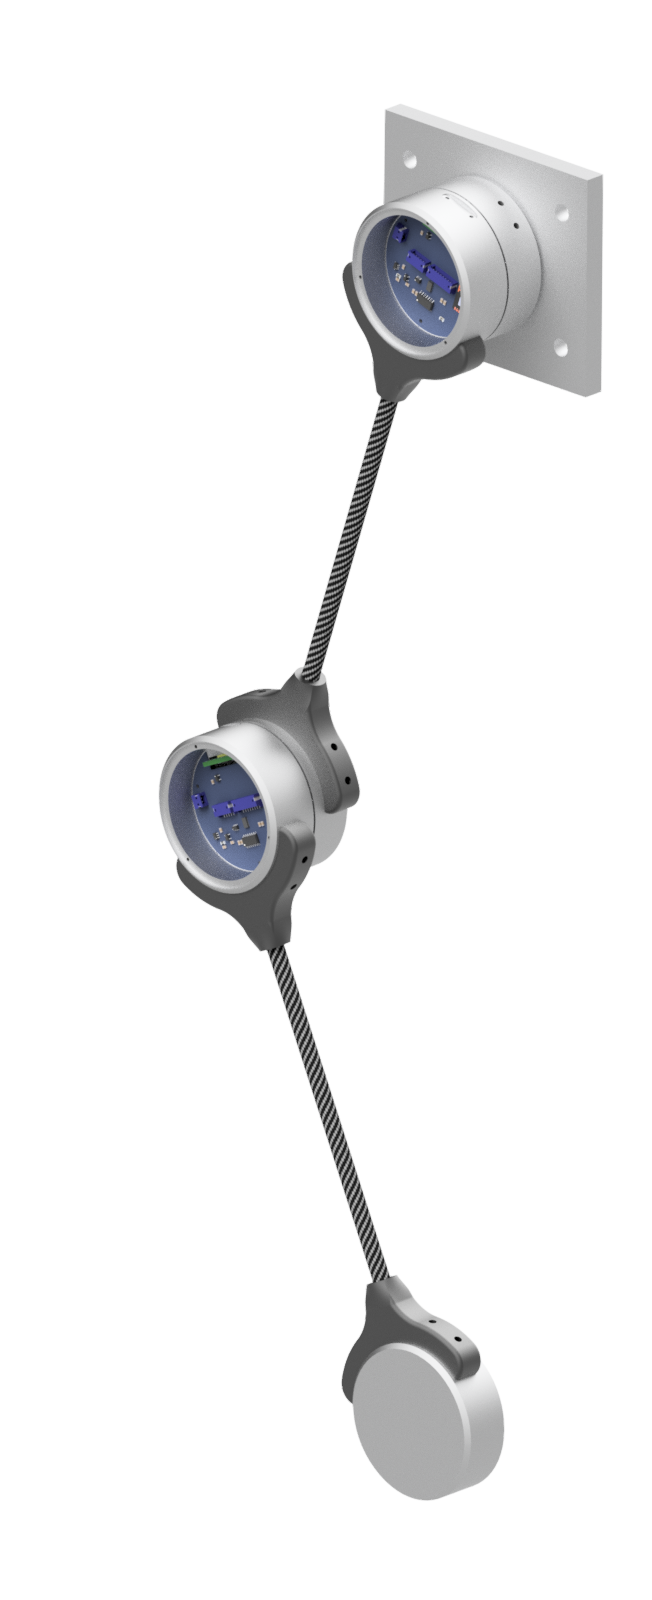
\includegraphics[width=.85\linewidth]{graphics/pendulum_assembly}
			\caption{This is a line of text}
			\label{sfig:pendulumassembly}
		\end{subfigure}\\
		\begin{subfigure}[b]{\linewidth}
			\centering
			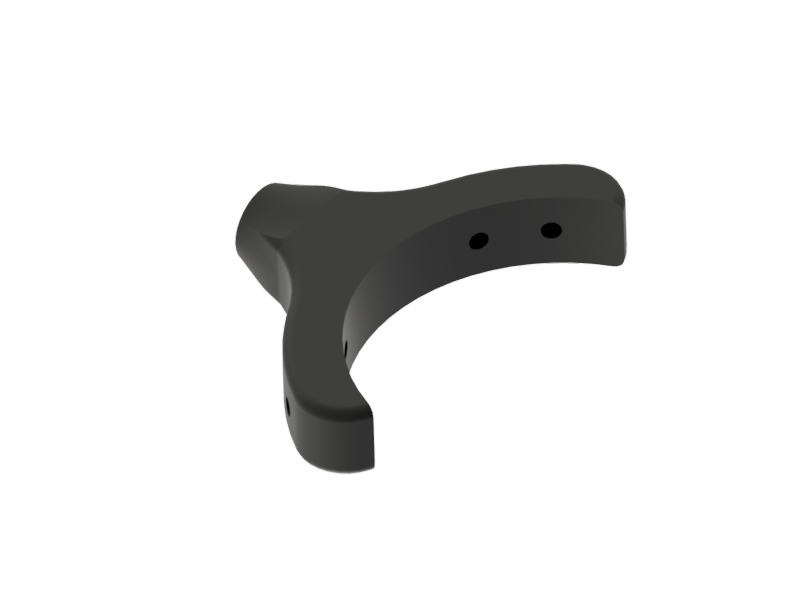
\includegraphics[width=\linewidth]{graphics/joint_mount}
			\caption{No one ever reads me... and some more text to fill out the caption}
			\label{sfig:jointmount}
		\end{subfigure}	
	\end{minipage}
	\begin{minipage}{.4\linewidth}
		\begin{subfigure}[t]{\linewidth}
			\centering
			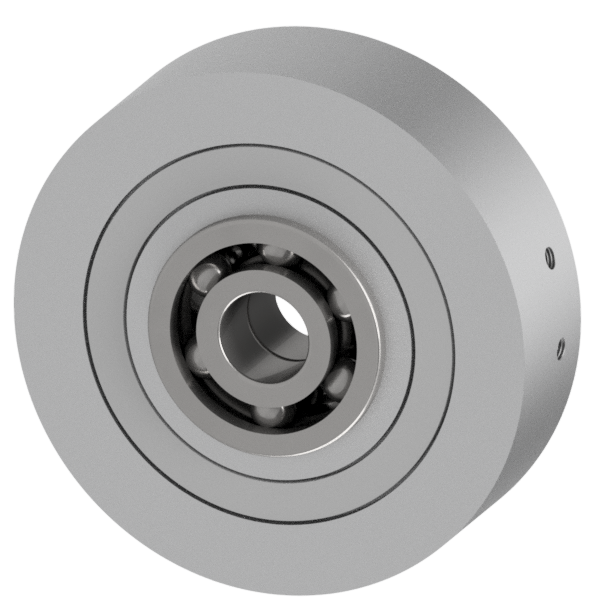
\includegraphics[width=\linewidth]{graphics/joint_mag_assembly}
			\caption{So is this..}
			\label{sfig:magnetside}
		\end{subfigure}\\
		\begin{subfigure}[b]{\linewidth}
			\centering
			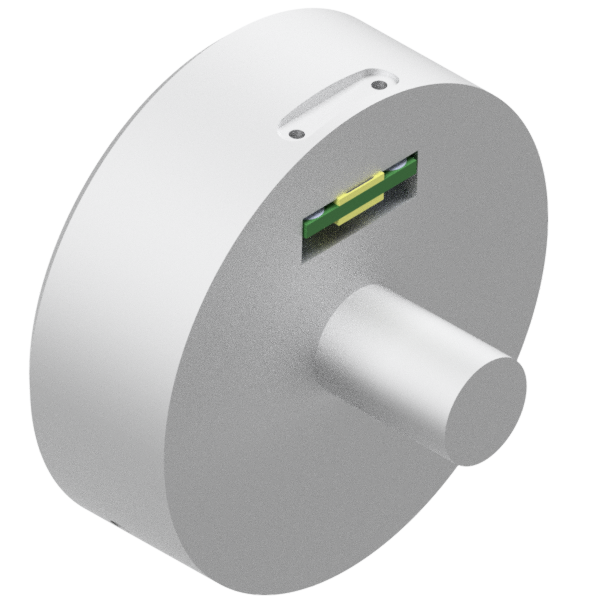
\includegraphics[width=\linewidth]{graphics/joint_read_side}
			\caption{And this!}
			\label{sfig:readside}
		\end{subfigure}\\
		\begin{subfigure}[b]{\linewidth}
			\centering
			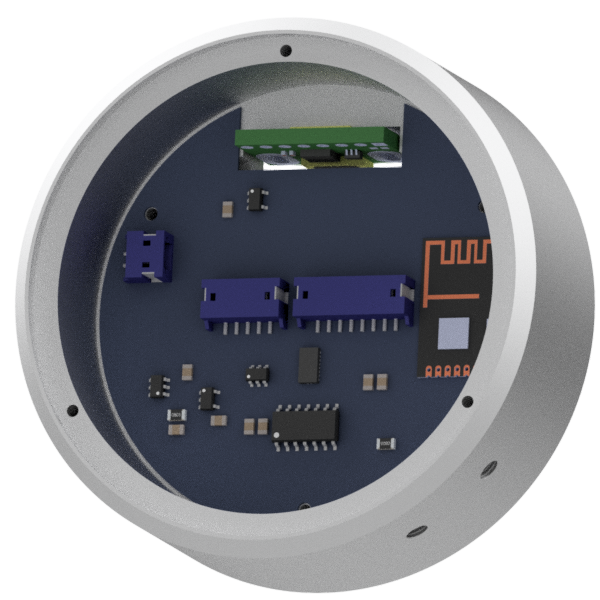
\includegraphics[width=\linewidth]{graphics/joint_read_side_2}
			\caption{Me too! this needs some more text as well. So here it is}
			\label{sfig:readside_2}
		\end{subfigure}
	\end{minipage}
	\caption{Me be Big-Momma Text!}
	\label{fig:mechdesign}
\end{figure}

\subsubsection{RS422}
The \texttt{RL2IC} uses the RS422 standard for its output.
This means that each \texttt{A}, \texttt{B} or \texttt{Z} channel consists of a two wire differential signal.
A line receiver is needed in order to translate the RS422 signals to logic inputs that the ATtiny84 can read.
The \texttt{DS26LS32CM} is a quad differential line receiver that complies with the RS422 standard.  
When using RS422 there are different termination methods, with no termination being the simplest.
The RS422 Standard Overview \cite{rs422_texas} describes that signal integrity is maintained in a setup of \approx 30m wires carrying data at a signal rate of 200kbps without termination.
The intended setup on the joint board requires wires no longer than 5cm.
The maximum expected data rate can be calculated using the maximum expected angular velocity of the joint of 20Hz and the edges on one channel per revolution.
\begin{equation}
Datarate_{max}	= 20 \cdot 3600 = 72kbps
\end{equation}
This datarate is clearly below the 200kbps and it was therefore decided to use no line termination, which also has the advantage that a minimum amount of current is needed from the \texttt{RL2IC}.


\subsubsection{5V}
As described in the requirements in section \ref{subs:joint_requirements}, a 5V rail is needed on the joint board.
Generating the 5V rail can be done by boosting the battery voltage up to 5V, as the battery voltage will always be lower than 5V.
The boost regulator \texttt{SP6641B} \cite{sp6641b} has an input range of 0.9V to 4.5V and a fixed output of 5V.
The circuitry used in this project will be based on the reference design shown in the datasheet, with the one difference that the \texttt{SHDN} (shutdown) pin has been pulled permanently high.

\subsubsection{3.3V}
A 3.3V rail is needed according to the requirement specification.
The task of generating the 3.3V rail is somewhat complicated since the battery voltage of a typical Li-Ion battery varies from 4.2V down to 3.0V.
Three different solutions appeared after an initial analysis of the task:

\begin{itemize}
	\item Buck converter
	\item Buck-Boost converter
	\item Linear regulator
\end{itemize}

The qualities and drawbacks of the three solutions are presented here.

\paragraph{Buck Converter:}
The voltage from the battery can be converted to 3.3V using a Buck converter.
A Buck converter is relatively simple and circuitry can easily be designed for the task.
It is only able to supply an output voltage that is lower than the input voltage.
Which means that when the battery voltage is lower than 3.3V the converter will stop producing a stable 3.3V output.
This means that a portion of the battery capacity cannot be used.
The \texttt{TPS62220} is a Buck regulator and generally has good specifications for this task. 
With an input voltage of 3.7V and an output voltage of 3.3V it has an efficiency of approximately 95\% with an output current in the range of 1mA to 20mA \cite{TPS6222}.
The minimum drop out voltage of the \texttt{TPS62220} is low, because it has a 100\% duty cycle mode.
In this mode, the the drop out voltage is purely defined by the \texttt{ON} resistance of the internal switch, the DC resistance of the external inductor and the output current.

The drop out voltage can be calculated using equation \ref{eq:drop_v_tps62}, \cite{TPS6222}.
\begin{equation}
	V_{drop} = I_{O} \cdot (R_{DS(on),max}+R_I)
	\label{eq:drop_v_tps62}
\end{equation}

\begin{equation}
	V_{drop} = 0.02 \cdot (0.67+0.09) = 15 [mV]
	\label{eq:drop_v_tps62_2}
\end{equation}

Where $I_O$ is the output current, $R_{DS(on),max}$ is the \texttt{ON} resistance of the internal switch and $R_I$ is the DC resistance of the external inductor.
The inductor resistance used is found in the \texttt{LQH55D} SMD inductor \cite{LQH55D}.
\mikkel{Update to new inductor and change equations above}
This means that it can supply 3.3V output when the input voltage is 3.315V or greater



\paragraph{Buck-Boost Converter:}
The motivation for using a Buck-Boost converter is to allow for full utilization of the battery capacity.
This requires that the converter can make a seamless transition between the stepping up and stepping down of the input voltage. 
\texttt{TPS6300} is a Buck-Boost regulator that has these features.
The external circuitry is simple, but the drawback of this regulator and converter is the efficiency of it.
With an input voltage of 3.7V and an output voltage of 3.3V it has an efficiency of approximately 75\% with an output current in the range of 1mA to 20mA \cite{TPS6300}.

\paragraph{Linear Regulator:}
A linear regulator is a component that can regulate the output voltage by varying an internal resistance.
Linear regulators have a drop voltage that limit the output voltage. 
The \texttt{LD3985} has an ultra low drop voltage of 20mV at 50mA output current \cite{LD3985}.

Therefore the efficiency is proportional to ratio between the output and input voltage and can be estimated using equation \ref{eq:eff_lin} \cite{ap_note_140}.

\begin{equation}
	\eta \simeq \frac{V_{out}}{V_{in}}
	\label{eq:eff_lin}
\end{equation}

The voltage of a Li-Ion battery varies from 4.2 to 3.0V, but the nominal voltage is 3.7V and this will be used as an estimate of the mean voltage of the battery.
Using this the mean efficiency can be estimated as shown in equation \ref{eq:eff_lin_val}.

\begin{equation}
	\eta \simeq \frac{3.3}{3.7} = 0.89 = 89\%
	\label{eq:eff_lin_val}
\end{equation}


\paragraph{Comparison}
The most important parameters of the three solutions discussed are shown in table \ref{tab:vol_gen_joint}.

\begin{table}[h]
	\centering
	\begin{tabular}{l|c|c|c}
		  				&	Buck 	& Buck-Boost 	& Linear\\
		 \hline
		 Efficiency  	&  95\% 	& 75\%			&89\%		\\
		 Drop out [mV]		&15  	& N/A		&20		\\
	\end{tabular}
	\caption[Parameters of voltage generation solutions.]{Parameters of the three solutions using a Buck converter, Buck-Boost converter or a linear regulator. The efficiency shown is estimated with an input voltage of 3.7V, an output voltage of 3.3V and an output current in the range of 1mA to 20mA. The drop out voltage is estimated with an output current of 20mA (Buck) and 50mA (linear regulator).}
	\label{tab:vol_gen_joint}
\end{table}

The Buck converter solution has the highest efficiency and is therefore the natural choice.
As already discussed the disadvantage of using a Buck converter is that the full battery capacity cannot be utilized.
A discharge test should be conducted to determine the amount of capacity that cannot be utilized.


\paragraph{Battery Discharge}
At the time of writing, the chosen battery has not yet been procured and the test will therefore be conducted on a similar battery instead.
The battery under test is a 850 mAH Li-Ion battery with the dimensions 49mm X 29mm X 6mm.
It should be noted that both the capacity and physical dimensions are similar to the chosen battery.
The discharge curve of the two batteries will not be identical, but will be sufficiently close to to allow for deciding which solution should be used.
The test was conducted by connecting the battery to an electrical load programmed to discharge with a constant power of 0.3 Watt, while measuring the battery voltage.
The measured discharge curve is shown in figure \ref{fig:bat_discharge}.

\begin{figure}[h]
	\centering
	%%% This file was created by matlab2tikz.
%
%The latest updates can be retrieved from
%  http://www.mathworks.com/matlabcentral/fileexchange/22022-matlab2tikz-matlab2tikz
%where you can also make suggestions and rate matlab2tikz.
%
\definecolor{mycolor1}{rgb}{0.00000,0.44700,0.74100}%
%
\begin{tikzpicture}

\begin{axis}[%
width=4.521in,
height=3.566in,
at={(0.758in,0.481in)},
scale only axis,
xmin=0,
xmax=450,
xlabel style={font=\color{white!15!black}},
xlabel={Time [Min]},
ymin=2.5,
ymax=4.5,
ytick={2.5,   3, 3.5,   4, 4.5},
ylabel style={font=\color{white!15!black}},
ylabel={Voltage [V]},
axis background/.style={fill=white},
title style={font=\bfseries},
title={Discharge Curve of Li-Ion Battery}
]
\addplot [color=mycolor1, forget plot]
  table[row sep=crcr]{%
0	4.072\\
10	4.02699999999999\\
20	4.00799999999998\\
40	3.95999999999998\\
50	3.92200000000003\\
60	3.89499999999998\\
70	3.87900000000002\\
80	3.85500000000002\\
90	3.84300000000002\\
100	3.81799999999998\\
110	3.79700000000003\\
120	3.78899999999999\\
130	3.77699999999999\\
140	3.767\\
150	3.75299999999999\\
160	3.76100000000002\\
170	3.75999999999999\\
180	3.74000000000001\\
190	3.72500000000002\\
200	3.71300000000002\\
210	3.714\\
220	3.69999999999999\\
230	3.71100000000001\\
240	3.71199999999999\\
250	3.69999999999999\\
260	3.69299999999998\\
270	3.69099999999997\\
280	3.69799999999998\\
290	3.69099999999997\\
300	3.68099999999998\\
310	3.673\\
320	3.65699999999998\\
330	3.64499999999998\\
340	3.63499999999999\\
350	3.62299999999999\\
360	3.60700000000003\\
370	3.61399999999998\\
380	3.596\\
390	3.56799999999998\\
400	3.505\\
410	3.36099999999999\\
414.551694551695	2.30000000000001\\
};
\addplot [color=red, dashed, forget plot]
  table[row sep=crcr]{%
0	3.30000000000001\\
450	3.30000000000001\\
};
\end{axis}
\end{tikzpicture}%
	\caption[Discharge curve of Li-Ion battery.]{Voltages measured across a 850 mAH Li-Ion battery while discharging using an electrical load programmed to 0.3 Watt. Horizontal red line represents the 3.3V level.}
	\label{fig:bat_discharge}
\end{figure}

It can be observed that the battery voltage only drops below 3.3V for a very short time before the battery is completely discharged.

\paragraph{Conclusion}
The Buck converter solution has the highest efficiency and has a lower drop out voltage than the linear regulator solution.
The disadvantage of using a Buck converter is that the full battery capacity cannot be utilized, but a test showed that almost all of the capacity can be used.
Therefore it was chosen to use a Buck converter with the \texttt{TPS62220} regulator. 
The Buck converter circuit used is based on the recommendations in the datasheet of the \texttt{TPS62220}.
The circuit is shown in figure \ref{fig:tps62220_circuit}.

\begin{figure}[h]
	\centering
    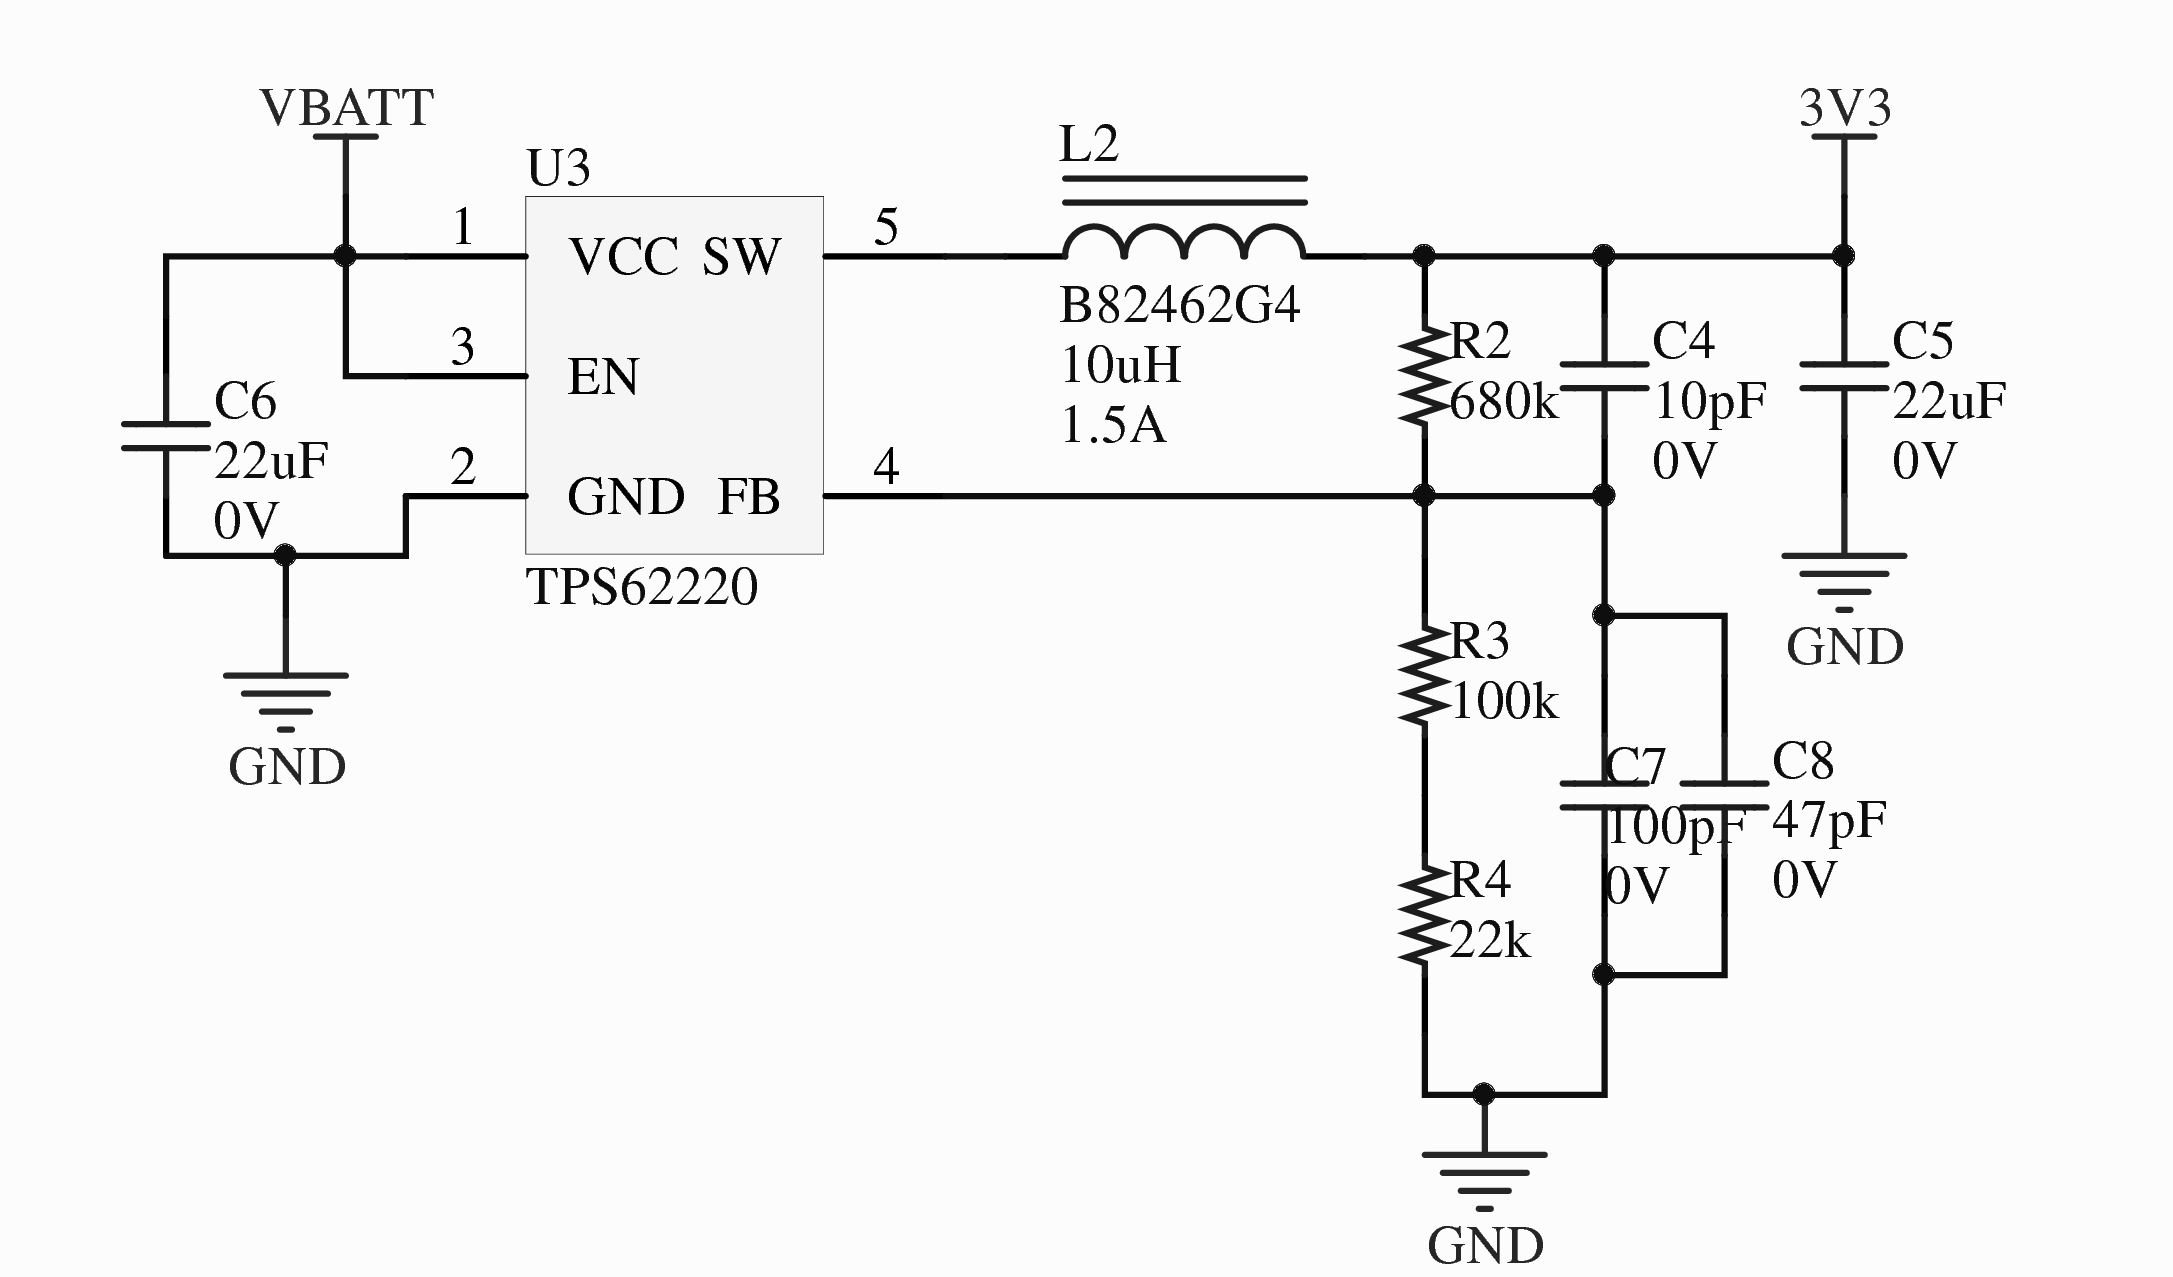
\includegraphics[width=.8\linewidth]{graphics/tps6220_circuit}
	\caption[3.3 V buck converter circuitry.]{Circuitry of Buck converter with an output voltage of 3.3V. \texttt{TPS62220} is used as the regulator.}
	\label{fig:tps62220_circuit}
\end{figure}
% subsection joint_design (end)

\subsubsection{Choosing a Battery} % (fold)
\label{ssub:choosing_a_battery}
It turned out to be rather difficult to procure a LiPo battery.
Apparently, they are in the habit of burning violently if damaged and for that reason, strict rules are in place concercing the transportation of them.
It was necessary to find a supplier with an appropriate battery who would also be willing to send them.
Eventually a danish distributor of Renata batteries was found.
Renata provides the \texttt{ICP582930PR-01} which is a 430mAH or 1600mWH.
This battery measures 32x29.5
\thomas{write few words on renata and difficulty of procurement (most capacity in 57mm and 9mm)}